\documentclass[12pt]{article}
\usepackage{pgfplots}
\begin{document}
\flushleft
\pgfplotsset{every axis legend/.append style={
legend columns=5,font=\small}}
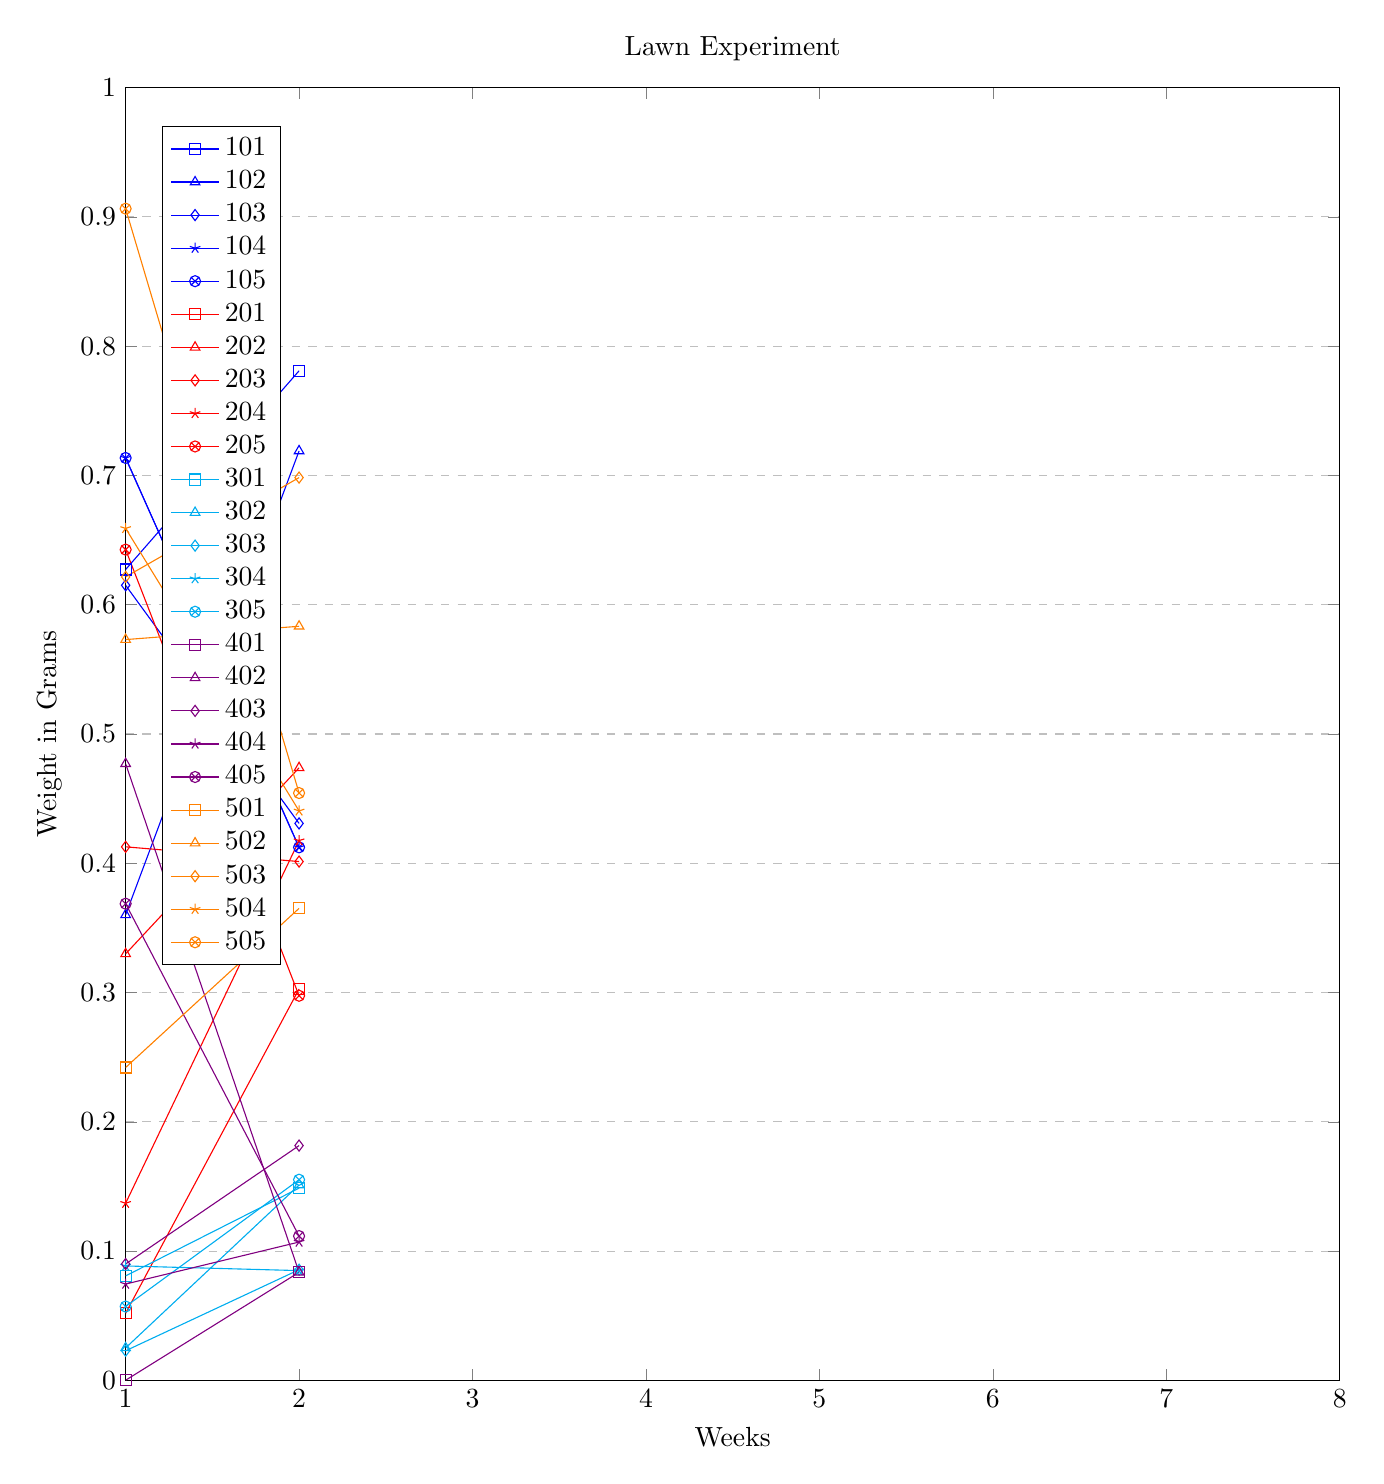
\begin{tikzpicture}
\begin{axis}[
width=17cm, height=18cm,     % size of the image
    title={Lawn Experiment},
    xlabel={Weeks},
    ylabel={Weight in Grams},
    xmin=1, xmax=8,
    ymin=0, ymax=1,
    xtick={1,2,3,4,5,6,7,8},
    ytick={0,.1,.2,.3,.4,.5,.6,.7,.8,.9,1},
    legend pos=north west,
    ymajorgrids=true,
    grid style=dashed,
]


\addplot[
%101
    color=blue,
    mark=square,
    ]
    coordinates {
    (1,0.6272)(2,0.7809)
    };
\addplot[
%102
    color=blue,
    mark=triangle,
    ]
    coordinates {
    (1,0.3601)(2,0.7189)
    };
\addplot[
%103
    color=blue,
    mark=diamond,
    ]
    coordinates {
    (1,0.615)(2,0.4308)
    };
\addplot[
%104
    color=blue,
    mark=star,
    ]
    coordinates {
    (1,0.7135)(2,0.4123)
    };
\addplot[
%105
    color=blue,
    mark=otimes,
    ]
    coordinates {
    (1,0.7135)(2,0.4123)
    };
\addplot[
%201
    color=red,
    mark=square,
    ]
    coordinates {
    (1,0.0519)(2,0.3027)
    };
\addplot[
%202
    color=red,
    mark=triangle,
    ]
    coordinates {
    (1,0.3299)(2,0.4738)
    };
\addplot[
%203
    color=red,
    mark=diamond,
    ]
    coordinates {
    (1,0.4127)(2,0.4013)
    };
\addplot[
%204
    color=red,
    mark=star,
    ]
    coordinates {
    (1,0.137)(2,0.4175)
    };
\addplot[
%205
    color=red,
    mark=otimes,
    ]
    coordinates {
    (1,0.6426)(2,0.2975)
    };
    \addplot[
%301
    color=cyan,
    mark=square,
    ]
    coordinates {
    (1,0.0808)(2,0.1487)
    };
\addplot[
%302
    color=cyan,
    mark=triangle,
    ]
    coordinates {
    (1,0.0251)(2,0.1511)
    };
\addplot[
%303
    color=cyan,
    mark=diamond,
    ]
    coordinates {
    (1,0.0229)(2,0.0856)
    };
\addplot[
%304
    color=cyan,
    mark=star,
    ]
    coordinates {
    (1,0.0885)(2,0.0849)
    };
\addplot[
%305
    color=cyan,
    mark=otimes,
    ]
    coordinates {
    (1,0.0571)(2,0.15519)
    };
        \addplot[
%401
    color=violet,
    mark=square,
    ]
    coordinates {
    (1,0.0001)(2,0.0836)
    };
\addplot[
%402
    color=violet,
    mark=triangle,
    ]
    coordinates {
    (1,0.477)(2,0.0836)
    };
\addplot[
%403
    color=violet,
    mark=diamond,
    ]
    coordinates {
    (1,0.09)(2,0.1816)
    };
\addplot[
%404
    color=violet,
    mark=star,
    ]
    coordinates {
    (1,0.0745)(2,0.107)
    };
\addplot[
%405
    color=violet,
    mark=otimes,
    ]
    coordinates {
    (1,0.3687)(2,0.1116)
    };
            \addplot[
%501
    color=orange,
    mark=square,
    ]
    coordinates {
    (1,0.242)(2,0.3651)
    };
\addplot[
%502
    color=orange,
    mark=triangle,
    ]
    coordinates {
    (1,0.573)(2,0.5833)
    };
\addplot[
%503
    color=orange,
    mark=diamond,
    ]
    coordinates {
    (1,0.6215)(2,0.6983)
    };
\addplot[
%504
    color=orange,
    mark=star,
    ]
    coordinates {
    (1,0.659)(2,0.4405)
    };
\addplot[
%505
    color=orange,
    mark=otimes,
    ]
    coordinates {
    (1,0.9063)(2,0.4543)
    };
    
    \legend{101,102,103,104,105,
            201,202,203,204,205,
            301,302,303,304,305,
            401,402,403,404,405,
            501,502,503,504,505}
 
\end{axis}

\end{tikzpicture}
\end{document}